\documentclass[]{article}
\usepackage{lmodern}
\usepackage{amssymb,amsmath}
\usepackage{ifxetex,ifluatex}
\usepackage{fixltx2e} % provides \textsubscript
\ifnum 0\ifxetex 1\fi\ifluatex 1\fi=0 % if pdftex
  \usepackage[T1]{fontenc}
  \usepackage[utf8]{inputenc}
\else % if luatex or xelatex
  \ifxetex
    \usepackage{mathspec}
    \usepackage{xltxtra,xunicode}
  \else
    \usepackage{fontspec}
  \fi
  \defaultfontfeatures{Mapping=tex-text,Scale=MatchLowercase}
  \newcommand{\euro}{€}
\fi
% use upquote if available, for straight quotes in verbatim environments
\IfFileExists{upquote.sty}{\usepackage{upquote}}{}
% use microtype if available
\IfFileExists{microtype.sty}{%
\usepackage{microtype}
\UseMicrotypeSet[protrusion]{basicmath} % disable protrusion for tt fonts
}{}
\ifxetex
  \usepackage[setpagesize=false, % page size defined by xetex
              unicode=false, % unicode breaks when used with xetex
              xetex]{hyperref}
\else
  \usepackage[unicode=true]{hyperref}
\fi
\hypersetup{breaklinks=true,
            bookmarks=true,
            pdfauthor={},
            pdftitle={},
            colorlinks=true,
            citecolor=blue,
            urlcolor=blue,
            linkcolor=magenta,
            pdfborder={0 0 0}}
\urlstyle{same}  % don't use monospace font for urls
\usepackage{color}
\usepackage{fancyvrb}
\newcommand{\VerbBar}{|}
\newcommand{\VERB}{\Verb[commandchars=\\\{\}]}
\DefineVerbatimEnvironment{Highlighting}{Verbatim}{commandchars=\\\{\}}
% Add ',fontsize=\small' for more characters per line
\newenvironment{Shaded}{}{}
\newcommand{\KeywordTok}[1]{\textcolor[rgb]{0.00,0.44,0.13}{\textbf{{#1}}}}
\newcommand{\DataTypeTok}[1]{\textcolor[rgb]{0.56,0.13,0.00}{{#1}}}
\newcommand{\DecValTok}[1]{\textcolor[rgb]{0.25,0.63,0.44}{{#1}}}
\newcommand{\BaseNTok}[1]{\textcolor[rgb]{0.25,0.63,0.44}{{#1}}}
\newcommand{\FloatTok}[1]{\textcolor[rgb]{0.25,0.63,0.44}{{#1}}}
\newcommand{\ConstantTok}[1]{\textcolor[rgb]{0.53,0.00,0.00}{{#1}}}
\newcommand{\CharTok}[1]{\textcolor[rgb]{0.25,0.44,0.63}{{#1}}}
\newcommand{\SpecialCharTok}[1]{\textcolor[rgb]{0.25,0.44,0.63}{{#1}}}
\newcommand{\StringTok}[1]{\textcolor[rgb]{0.25,0.44,0.63}{{#1}}}
\newcommand{\VerbatimStringTok}[1]{\textcolor[rgb]{0.25,0.44,0.63}{{#1}}}
\newcommand{\SpecialStringTok}[1]{\textcolor[rgb]{0.73,0.40,0.53}{{#1}}}
\newcommand{\ImportTok}[1]{{#1}}
\newcommand{\CommentTok}[1]{\textcolor[rgb]{0.38,0.63,0.69}{\textit{{#1}}}}
\newcommand{\DocumentationTok}[1]{\textcolor[rgb]{0.73,0.13,0.13}{\textit{{#1}}}}
\newcommand{\AnnotationTok}[1]{\textcolor[rgb]{0.38,0.63,0.69}{\textbf{\textit{{#1}}}}}
\newcommand{\CommentVarTok}[1]{\textcolor[rgb]{0.38,0.63,0.69}{\textbf{\textit{{#1}}}}}
\newcommand{\OtherTok}[1]{\textcolor[rgb]{0.00,0.44,0.13}{{#1}}}
\newcommand{\FunctionTok}[1]{\textcolor[rgb]{0.02,0.16,0.49}{{#1}}}
\newcommand{\VariableTok}[1]{\textcolor[rgb]{0.10,0.09,0.49}{{#1}}}
\newcommand{\ControlFlowTok}[1]{\textcolor[rgb]{0.00,0.44,0.13}{\textbf{{#1}}}}
\newcommand{\OperatorTok}[1]{\textcolor[rgb]{0.40,0.40,0.40}{{#1}}}
\newcommand{\BuiltInTok}[1]{{#1}}
\newcommand{\ExtensionTok}[1]{{#1}}
\newcommand{\PreprocessorTok}[1]{\textcolor[rgb]{0.74,0.48,0.00}{{#1}}}
\newcommand{\AttributeTok}[1]{\textcolor[rgb]{0.49,0.56,0.16}{{#1}}}
\newcommand{\RegionMarkerTok}[1]{{#1}}
\newcommand{\InformationTok}[1]{\textcolor[rgb]{0.38,0.63,0.69}{\textbf{\textit{{#1}}}}}
\newcommand{\WarningTok}[1]{\textcolor[rgb]{0.38,0.63,0.69}{\textbf{\textit{{#1}}}}}
\newcommand{\AlertTok}[1]{\textcolor[rgb]{1.00,0.00,0.00}{\textbf{{#1}}}}
\newcommand{\ErrorTok}[1]{\textcolor[rgb]{1.00,0.00,0.00}{\textbf{{#1}}}}
\newcommand{\NormalTok}[1]{{#1}}
\usepackage{graphicx,grffile}
\makeatletter
\def\maxwidth{\ifdim\Gin@nat@width>\linewidth\linewidth\else\Gin@nat@width\fi}
\def\maxheight{\ifdim\Gin@nat@height>\textheight\textheight\else\Gin@nat@height\fi}
\makeatother
% Scale images if necessary, so that they will not overflow the page
% margins by default, and it is still possible to overwrite the defaults
% using explicit options in \includegraphics[width, height, ...]{}
\setkeys{Gin}{width=\maxwidth,height=\maxheight,keepaspectratio}
\setlength{\parindent}{0pt}
\setlength{\parskip}{6pt plus 2pt minus 1pt}
\setlength{\emergencystretch}{3em}  % prevent overfull lines
\providecommand{\tightlist}{%
  \setlength{\itemsep}{0pt}\setlength{\parskip}{0pt}}
\setcounter{secnumdepth}{0}

\date{}

% Redefines (sub)paragraphs to behave more like sections
\ifx\paragraph\undefined\else
\let\oldparagraph\paragraph
\renewcommand{\paragraph}[1]{\oldparagraph{#1}\mbox{}}
\fi
\ifx\subparagraph\undefined\else
\let\oldsubparagraph\subparagraph
\renewcommand{\subparagraph}[1]{\oldsubparagraph{#1}\mbox{}}
\fi

\begin{document}

\section{Goals}\label{goals}

\begin{itemize}
\tightlist
\item
  To understand what is image filtering
\item
  Learn about various available image filters in python.
\item
  Learn to code for Gaussian, box and median filters.
\end{itemize}

\section{Theory}\label{theory}

Image blurring is achieved by convolving the image with a low-pass
filter kernel. It is useful for removing noise. It actually removes high
frequency content (e.g: noise, edges) from the image resulting in edges
being blurred when this is filter is applied. We will discuss three such
filters: * Blur filter * Gaussian filter * Median Blur filter

\subsection{Blur}\label{blur}

\subsubsection{Working Principle}\label{working-principle}

Also known as Averaging, this technique uses a normalized box filter to
convolve images. The low-pass filter kernel is positioned in the image
such that it is a subset of the image. The pixel lying in the center of
the kernel will get its value calculated. All the pixels in the kernel
area will be used to find the average, which is assigned as the new
value of the central pixel. This is an example of a normalized box
filter-

\begin{figure}[htbp]
\centering
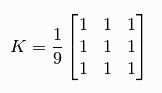
\includegraphics{Blur_kernel.png}
\caption{Blur Kernel}
\end{figure}

The following function is used to blur an image:

\begin{Shaded}
\begin{Highlighting}[]
\NormalTok{cv2.blur( src, ksize[, dst[, anchor[, borderType]]])}
\end{Highlighting}
\end{Shaded}

\subsubsection{Parameters:}\label{parameters}

\begin{itemize}
\tightlist
\item
  \textbf{src} - Input image that can have any number of input channels.
  The depth should be CV\_8U, CV\_16U, CV\_16S, CV\_32F or CV\_64F.\\
\item
  \textbf{ksize} - Size of kernel used for blurring\\
\item
  \textbf{dst} - Output image of the same size and type as src.\\
\item
  \textbf{anchor} - Anchor point; default value Point(-1,-1) means that
  the anchor is at the kernel center.
\item
  \textbf{borderType} - Border mode used to extrapolate pixels outside
  the image.
\end{itemize}

\subsection{Gaussian Blur}\label{gaussian-blur}

\subsubsection{Working Principle}\label{working-principle-1}

In this method, a Gaussian kernel is used for filtering. Gaussian filter
is a low pass filter. It is done by convolving each point in the input
array with a Gaussian kernel and then summing them all up to produce the
output array.\\
Gaussian filtering is linear, meaning it replaces each pixel by a linear
combination of its neighbors (in this case with weights specified by a
Gaussian matrix). It is also local, meaning it produces output pixel
values based only upon the pixel values in its neighborhood as
determined by the convolution kernel. We should specify the width and
height of the kernel which should be positive and odd.\\
Here is an example of 5x5 Gaussian kernel:

\begin{figure}[htbp]
	\centering
    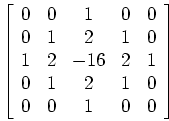
\includegraphics{Gaussian Kernel.png}
    \caption{Gaussian Kernel}
\end{figure}

The value of the pixel obtained on evaluating all the pixel values of
the neighborhood using the Gaussian function may not be present in the
image itself. Hence it results in some blurring. It is also not edge
preserving.\\
A 2D Gaussian function is as given below:

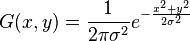
\includegraphics{Gaussfunc.png}\\
\\
Gaussian kernel coefficients are sampled using the above function. For
perfect filtering medianblur() is preferred.

The Gaussian blur can be applied to the images by the following
function:

\texttt{cv2.GaussianBlur(\ src,\ ksize,\ sigmaX,\ dst,\ sigmaY,\ borderType)}\\

\large Parameters : \\
* \textbf{src} - Input image; the image can have any number of channels,
which are processed independently, but the depth should be CV\_8U,
CV\_16U, CV\_16S, CV\_32F or CV\_64F.\\
* \textbf{ksize} - Gaussian kernel size.\\
* \textbf{sigmaX} - Gaussian kernel standard deviation in X direction.\\
* \textbf{dst} - Output image of the same size and type as src.\\
* \textbf{sigmaY} - Gaussian kernel standard deviation in Y direction;
if sigmaY is zero, it is set to be equal to sigmaX.\\
* \textbf{borderType} - Pixel extrapolation method

\subsection{Median Blur}\label{median-blur}

In this type, the central pixel's value is calculated by finding the
median of the pixel values in the kernel areas. Median refers to the
central value in a given set of values. Median blur differs from
Gaussian and box filters in one aspect- The central element is always
replaced by a pixel value that is present in the image. In the other
filters, filtered value for central element may be a value that is not
present in the original image. This property of Median Blur reduces
noise effectively.

The function used for median blur is-

\begin{Shaded}
\begin{Highlighting}[]
\NormalTok{cv2.medianBlur(src, ksize[, dst])}
\end{Highlighting}
\end{Shaded}

\subsubsection{Parameters:}\label{parameters-1}

\begin{itemize}
\tightlist
\item
  \textbf{src} - Input 1-, 3-, or 4-channel image; when ksize is 3 or 5,
  the image depth should be CV\_8U, CV\_16U, or CV\_32F, for larger
  aperture sizes, it can only be CV\_8U.
\item
  \textbf{ksize} - Aperture linear size; it must be odd and greater than
  1.
\item
  \textbf{dst} - Destination array of the same size and type as src.
\end{itemize}

\subsection{Applications:}\label{applications}

\begin{itemize}
\tightlist
\item
  These filters are used in edge detection.\\
\item
  They effective in smoothening images.
\item
  They can remove noise(like salt and pepper noise) from an image.
\end{itemize}

\section{Code}\label{code}

\subsection{Blur}\label{blur-1}

\begin{Shaded}
\begin{Highlighting}[]
    \CommentTok{#Imports}
    \ImportTok{import} \NormalTok{cv2}
    \ImportTok{from} \NormalTok{matplotlib }\ImportTok{import} \NormalTok{pyplot }\ImportTok{as} \NormalTok{plt}
    
    \CommentTok{#Read image}
    \NormalTok{img }\OperatorTok{=} \NormalTok{cv2.imread(}\StringTok{'example.jpg'}\NormalTok{)}

    \CommentTok{#Blur the image}
    \NormalTok{blur }\OperatorTok{=} \NormalTok{cv2.blur(img, (}\DecValTok{5}\NormalTok{,}\DecValTok{5}\NormalTok{))}

    \CommentTok{#Plot both images and compare}
    \NormalTok{plt.figure(}\DecValTok{0}\NormalTok{)}
    
    \NormalTok{plt.subplolt(}\DecValTok{121}\NormalTok{) }\CommentTok{#In a grid of 1 row and 2 columns, use first subplot}
    \NormalTok{plt.imshow(img), plt.title(}\StringTok{'Original'}\NormalTok{)}
    \NormalTok{plt.xticks([]), plt.yticks([]) }\CommentTok{#Remove ticks}

    \NormalTok{plt.subplot(}\DecValTok{122}\NormalTok{) }\CommentTok{#Use second subplot}
    \NormalTok{plt.imshow(blur), plt.title(}\StringTok{'Blurred'}\NormalTok{)}
    \NormalTok{plt.xticks([]), plt.yticks([])}

    \NormalTok{plt.show()}
\end{Highlighting}
\end{Shaded}

Consider the following image:

\begin{figure}[htbp]
\centering

\includegraphics{dots.jpg}
\caption{Example image}
\end{figure}

On applying blur, it looks like this-

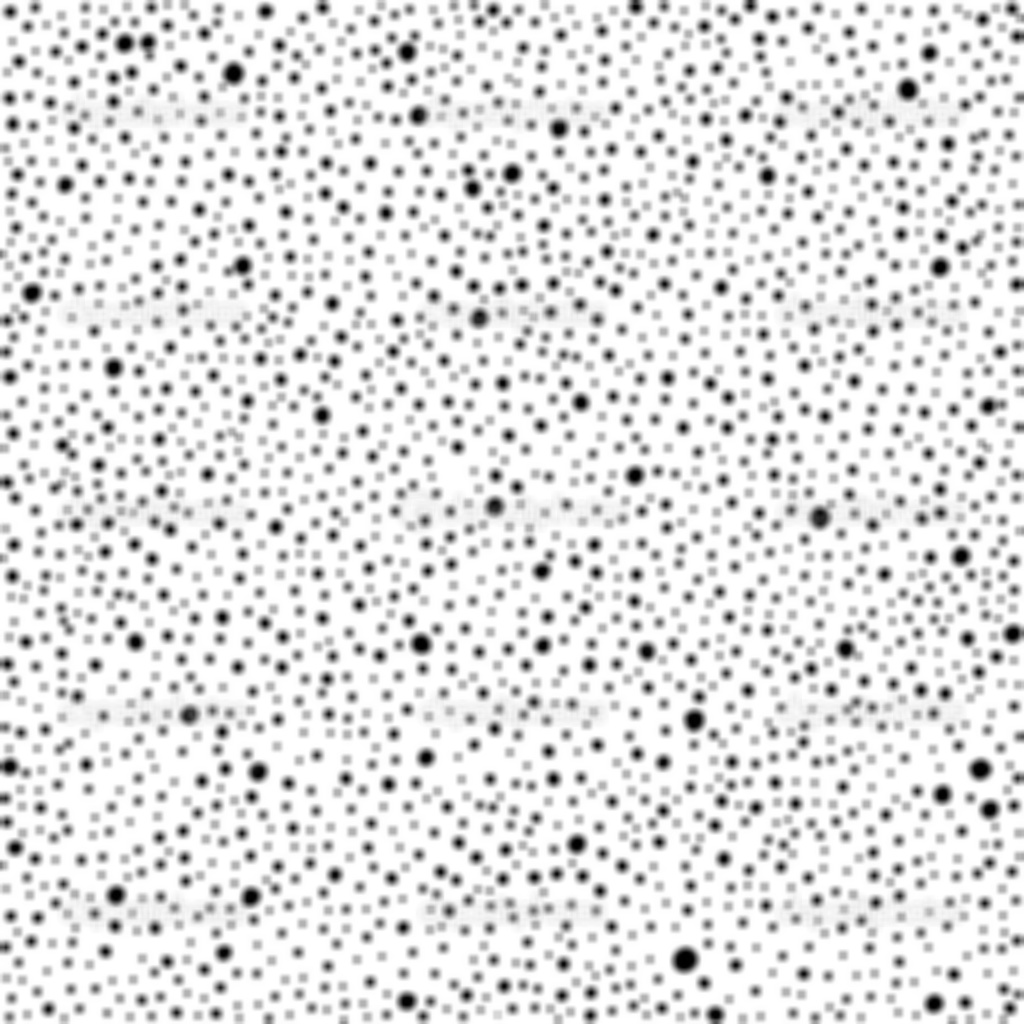
\includegraphics{Blur.jpg}
\#\#Gaussian Blur

\begin{verbatim}
  #Import OpenCV and Numpy
  import numpy
  import cv2

  #Read the image
  img = cv2.imread('pepper.png')

  '''
  OpenCV represents RGB images as multi-dimensional NumPy arrays…but in reverse
  order!This means that images are actually represented in BGR order rather than
  RGB!
  '''
  img = cv2.cvtColor(img, cv2.COLOR_BGR2RGB)   #Coverting from bgr to rgb

  # Do the processing
  blur = cv2.GaussianBlur(img,(5,5),0)

  plt.figure(0)       # Create a new window

  plt.subplot(121),plt.imshow(img), plt.title('Original')
  plt.xticks([]), plt.yticks([])      #Removing ticks

  plt.subplot(122),plt.imshow(blur), plt.title('Gaussian')
  plt.xticks([]), plt.yticks([])

  plt.show()          #Display the window
\end{verbatim}

\begin{figure}[htbp]
\centering
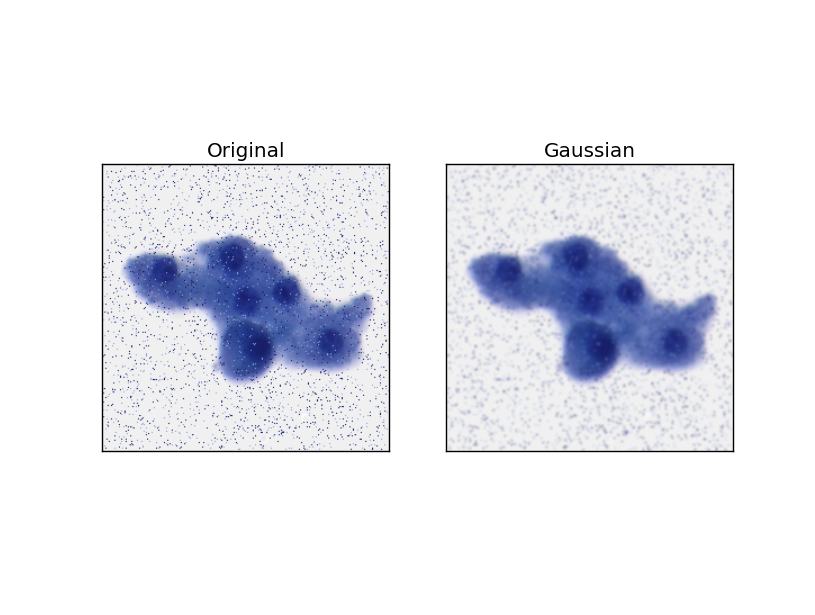
\includegraphics{GaussBlur.png}
\caption{Gauss Image}
\end{figure}

\subsection{Median Blur}\label{median-blur-1}

\begin{Shaded}
\begin{Highlighting}[]
    \CommentTok{#Imports}
    \ImportTok{import} \NormalTok{cv2}
    \ImportTok{from} \NormalTok{matplotlib }\ImportTok{import} \NormalTok{pyplot }\ImportTok{as} \NormalTok{plt}
    
    \CommentTok{#Read image}
    \NormalTok{img }\OperatorTok{=} \NormalTok{cv2.imread(}\StringTok{'example.jpg'}\NormalTok{)}

    \CommentTok{#Apply median blur}
     \NormalTok{mBlur }\OperatorTok{=} \NormalTok{cv2.medianBlur(img, }\DecValTok{5}\NormalTok{)}

    \CommentTok{#Plot both images and compare}
    \NormalTok{plt.figure(}\DecValTok{0}\NormalTok{)}
    
    \NormalTok{plt.subplolt(}\DecValTok{121}\NormalTok{) }\CommentTok{#In a grid of 1 row and 2 columns, use first subplot}
    \NormalTok{plt.imshow(img), plt.title(}\StringTok{'Original'}\NormalTok{)}
    \NormalTok{plt.xticks([]), plt.yticks([]) }\CommentTok{#Remove ticks}

    \NormalTok{plt.subplot(}\DecValTok{122}\NormalTok{) }\CommentTok{#Use second subplot}
    \NormalTok{plt.imshow(mBlur), plt.title(}\StringTok{'Blurred'}\NormalTok{)}
    \NormalTok{plt.xticks([]), plt.yticks([])}

    \NormalTok{plt.show()}
\end{Highlighting}
\end{Shaded}

Consider the following image-

\begin{figure}[htbp]
\centering
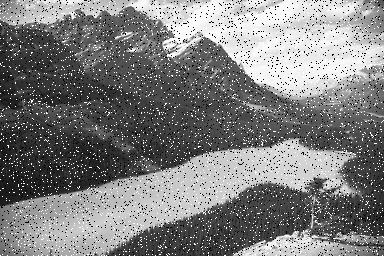
\includegraphics{mountains.png}
\caption{Example image}
\end{figure}

On apply median blur, it looks like this-

\begin{figure}[htbp]
\centering
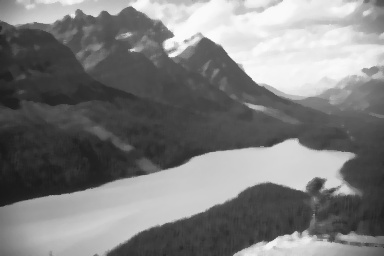
\includegraphics{Median.jpg}
\caption{Median Image}
\end{figure}

\newpage
\section{Resources}\label{resources}

\begin{itemize}
\tightlist
\item
  http://opencv-python-tutroals.readthedocs.org/en/latest/py\_tutorials/py\_imgproc/py\_filtering/py\_filtering.html
\item
  http://docs.opencv.org/modules/imgproc/doc/filtering.html\#
\end{itemize}

\section{Exercises}\label{exercises}

\end{document}
